\subsection*{Teil B: Projektaufgabe - Schulhofgestaltung (70 Minuten)}

\textbf{Situation:} Eure Schule plant eine neue Pausenhofgestaltung. Ihr sollt verschiedene Bereiche planen und berechnen.

\begin{enumerate}[label=\arabic*.,resume]

    \item \textbf{Sportplatz (Vierecke) - 20 Minuten}

    Der rechteckige Sportplatz soll 25 m × 15 m groß werden. In einer Ecke wird ein quadratisches Basketballfeld mit 8 m Seitenlänge eingerichtet.

    \begin{enumerate}[label=\alph*)]
        \item Zeichne einen Lageplan (Maßstab 1:500):

        \vspace{4cm}

        \item Berechne die Gesamtfläche des Sportplatzes:

        \vspace{1.5cm}

        \item Berechne die Fläche des Basketballfeldes:

        \vspace{1.5cm}

        \item Wie groß ist die restliche Sportfläche?

        \vspace{1.5cm}

        \item Wie viele Meter Zaun werden für die Umzäunung benötigt?

        \vspace{1.5cm}

    \end{enumerate}

    \item \textbf{Pausenverkauf (Funktionen) - 20 Minuten}

    Die Schule plant einen Pausenverkauf. Die Kosten setzen sich zusammen aus:
    - Fixkosten: 50 € pro Tag
    - Variable Kosten: 1,20 € pro verkauftem Brötchen
    - Verkaufspreis: 2,50 € pro Brötchen

    \begin{enumerate}[label=\alph*)]
        \item Stelle die Kostenfunktion auf: $K(x) = $ \underline{\hspace{6cm}}

        \item Stelle die Erlösfunktion auf: $E(x) = $ \underline{\hspace{6cm}}

        \item Berechne den Break-Even-Point (Gewinngrenze):

        \vspace{3cm}

        \item Zeichne beide Funktionen in ein Koordinatensystem:

        \begin{center}
            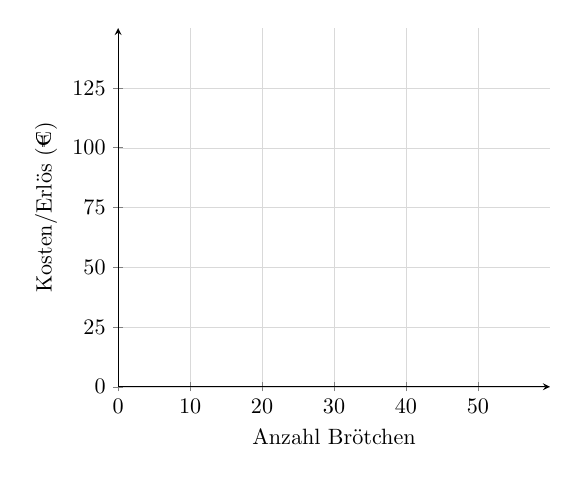
\begin{tikzpicture}[scale=0.8]
                \begin{axis}[
                    axis lines = left,
                    xlabel = {Anzahl Brötchen},
                    ylabel = {Kosten/Erlös (€)},
                    xmin=0, xmax=60,
                    ymin=0, ymax=150,
                    xtick={0,10,20,30,40,50},
                    ytick={0,25,50,75,100,125},
                    grid=major,
                    grid style={line width=0.1pt,draw=gray!30},
                ]
                \end{axis}
            \end{tikzpicture}
        \end{center}

        \item Wie hoch ist der Gewinn bei 50 verkauften Brötchen?

        \vspace{2cm}

    \end{enumerate}

    \item \textbf{Wasserspiele (Gleichungen) - 15 Minuten}

    Für ein kleines Wasserspiel wird ein zylindrischer Tank benötigt. Der Tank hat einen Durchmesser von 2 m und fasst 6280 Liter.

    \begin{enumerate}[label=\alph*)]
        \item Berechne die Höhe des Tanks:

        \textit{Hinweis:} $V = \pi r^2 h$ und $1 \text{ m}^3 = 1000 \text{ Liter}$

        \vspace{3cm}

        \item Der Tank wird mit 150 Litern pro Minute gefüllt. Nach wie vielen Minuten ist er voll?

        \textit{Gleichung aufstellen und lösen:}

        \vspace{3cm}

    \end{enumerate}

    \item \textbf{Sitzgelegenheiten (Raumgeometrie) - 15 Minuten}

    Es sollen zylindrische Sitzsäulen aus Beton aufgestellt werden. Jede Säule hat einen Durchmesser von 50 cm und eine Höhe von 45 cm.

    \begin{enumerate}[label=\alph*)]
        \item Berechne das Volumen einer Sitzsäule:

        \vspace{2cm}

        \item Wie viel Beton wird für 8 Sitzsäulen benötigt?

        \vspace{1.5cm}

        \item Berechne die Oberfläche einer Säule (inklusive Boden, ohne Deckel):

        \vspace{2.5cm}

        \item 1 m² Oberfläche kostet 25 € zum Beschichten. Was kosten alle 8 Säulen?

        \vspace{2cm}

    \end{enumerate}

\end{enumerate}